\subsection{Понятие k-мерного Евклидова пространства} \label{sec:1.1}

Рассмотрим множество $\displaystyle \mathbb{R}^k = \mathbb{R \cdot R \cdot ... \cdot R}$ упорядоченных наборов действительных чисел длины $k$ $(x_1, x_2, ..., x_k)$, где $x_1 \in \mathbb R$, $x_2 \in \mathbb R$, ..., $x_k \in \mathbb R$.

Упорядоченный набор $(x_1, x_2, ..., x_k)$ называется \textbf{точкой} или \textbf{вектором на множестве} $\mathbb{R}^k$ и обозначается $\vec{x} = (x_1, x_2, ..., x_k)$, а действительные числа $x_1, x_2, ..., x_k$ называются координатными векторами или точками.\\

Пусть $k=2$, тогда множество $\mathbb{R}^k$ определяет плоскость \cref{fig:1.1.1.1}. Координаты любой точки на плоскости — это упорядоченная пара чисел $(x_1, x_2)$, эта пара чисел является координатами вектора, проведенного из начала координат в данную точку.

\begin{figure}[H]
	\centering
	\begin{minipage}{0.45\linewidth}
		\centering
		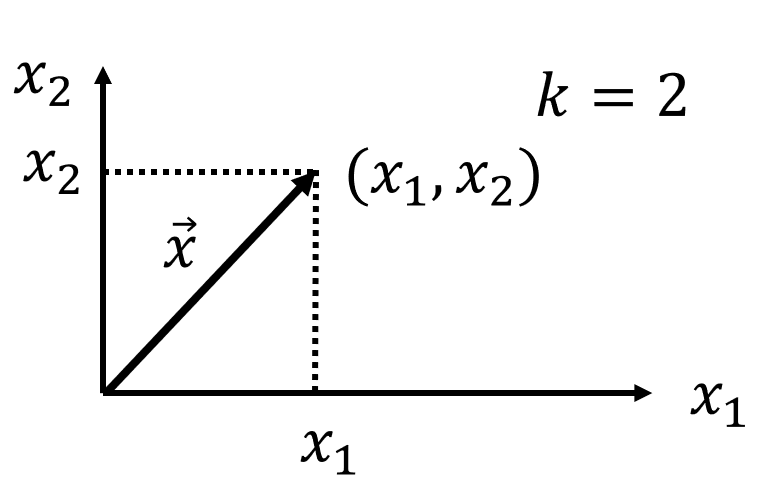
\includegraphics[width=0.9\linewidth]{image/screenshot001.png}
		\subcaption{При $k=2$}
		\label{fig:1.1.1.1}
	\end{minipage}
	\begin{minipage}{0.45\linewidth}
		\centering
		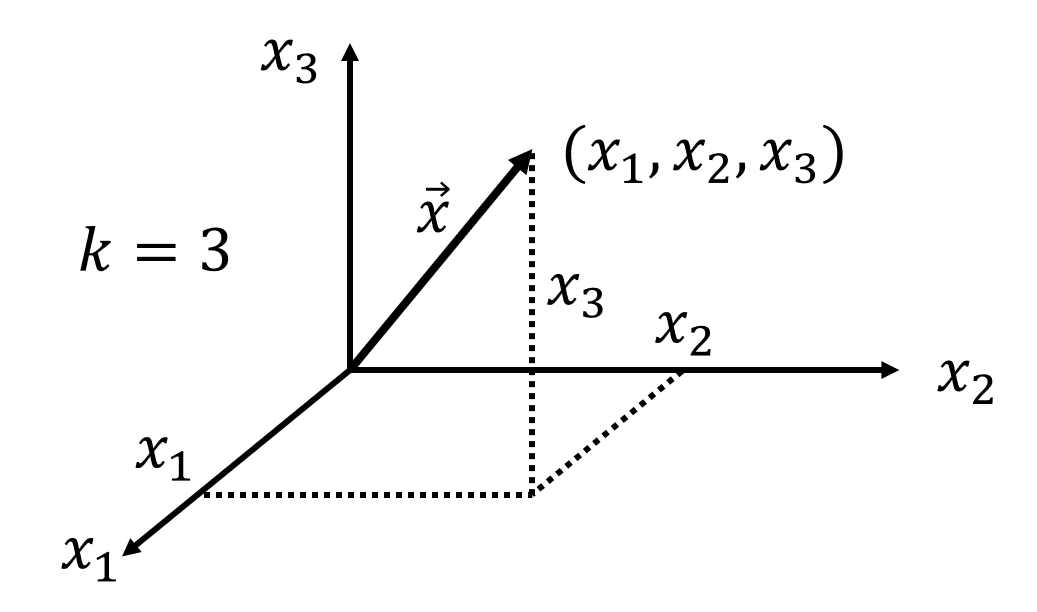
\includegraphics[width=0.9\linewidth]{image/screenshot006.png}
		\subcaption{При $k=3$}
		\label{fig:1.1.1.2}
	\end{minipage}
	\caption{Примеры $\mathbb{R}^k$ пространств}
	\label{fig:1.1.1}
\end{figure}

Аналогично, если $k=3$, то упорядоченный набор $(x_1, x_2, x_3)$ определяет точку или вектор в пространстве (\Cref{fig:1.1.1.2}).

Таким образом, элементами множества $\mathbb{R}^k$ являются \uline{векторы}. Над векторами вводятся следующие операции:
\begin{enumerate}
	\item \textbf{Сложение векторов}\\
	Если $\vec{x} = (x_1, x_2, ..., x_k) \in \mathbb{R}^k$ и $\vec{y} = (y_1, y_2, ..., y_k) \in \mathbb{R}^k$, то суммой векторов $(\vec{x} + \vec{y})$, будет являться сумма соответствующих координат:
	\begin{align} \label{1.1.1}
		(\vec{x} + \vec{y}) = (x_1 + y_1, x_2 + y_2, ..., x_k + y_k)
	\end{align}

	\item \textbf{Умножение вектора на скаляр}\\
	Если $\vec{x} = (x_1, x_2, ..., x_k)$ и $\alpha \in \mathbb R$ - действительное число, то $\alpha \vec{x} \in \mathbb{R}^k$ -- это вектор с координатами:
	\begin{align} \label{eq:1.1.2}
		(\alpha\vec{x}) = (\alpha \cdot x_1, \alpha \cdot x_2, ..., \alpha \cdot x_k)
	\end{align}

	\item \textbf{Скалярное произведение векторов}\\
	Если $\vec{x} = (x_1, x_2, ..., x_k) \in \mathbb{R}^k$ и $\vec{y} = (y_1, y_2, ..., y_k) \in \mathbb{R}^k$, тогда \textit{скалярным произведением векторов} называться скалярная величина, равная сумме произведений одноименных координат:
	\begin{align} \label{eq:1.1.3}
		(\vec{x} + \vec{y}) = x_1 y_1 + x_2 y_2 + ... + x_k y_k = \sum_{i = 1}^{k} x_i y_i
	\end{align}

	\item \textbf{Норма или длина вектора}\\
	Длина вектора $\vec{x} = (x_1, x_2, ..., x_k)$ вычисляется по формуле:
	\begin{align} \label{eq:1.1.4}
		||\vec{x}|| = \sqrt{x_1^2 + x_2^2 + ... + x_k^2} = \sqrt{\sum_{i=1}^{k} x_i^2}
	\end{align}

	\item \textbf{Расстояние между двумя точками или векторами}\\
	Если $\vec{x} = (x_1, x_2, ..., x_k) \in \mathbb{R}^k$ и $\vec{y} = (y_1, y_2, ..., y_k) \in \mathbb{R}^k$, то расстояние между точками $\rho(\vec{x}, \vec{y})$ определяется длиной вектора $(\vec{x} - \vec{y})$:
	\begin{multline} \label{eq:1.1.5}
		\rho(\vec{x}, \vec{y}) = ||\vec{x} - \vec{y}|| = \sqrt{(x_1 - y_1)^2 + (x_2 - y_2)^2 + ... + (x_k - y_k)^2} = \\ = \sqrt{\sum_{i=1}^{k} (x_i - y_i)^2}
	\end{multline}
\end{enumerate}

Если в множестве $\mathbb{R}^k$ введены рассмотренные выше операции с векторами, то оно называется \textbf{k-мерным Евклидовым пространством}.